\documentclass[11pt]{article}

\usepackage[a4paper, margin=1in]{geometry}
\usepackage[utf8]{inputenc}
\usepackage[T1]{fontenc}
\usepackage{microtype}
\usepackage{amsmath, amssymb, amsthm}
\usepackage{booktabs}
\usepackage{multirow}
\usepackage{graphicx}
\usepackage{hyperref}
\usepackage{natbib}
\usepackage{authblk}
\usepackage{float}
\usepackage{xcolor}

\hypersetup{
  colorlinks=true,
  linkcolor=blue!50!black,
  citecolor=blue!50!black,
  urlcolor=blue!50!black,
}

\title{\bf Directional Accuracy in Limit Order Book Prediction: \\
Sequence Models vs Tabular ML on BTC/USDT}

\author[1]{Manav Mishra\thanks{\texttt{manavmishra260205@gmail.com}}}
\affil[1]{Vellore Institute of Technology, Vellore, India}

\date{\today}

\begin{document}

\maketitle

\begin{abstract}
Limit order book (LOB) direction prediction is dominated by a small
number of order-flow imbalance (OFI) features whose relationship to
short-horizon mid-price changes is largely linear
\citep{cont2014price}. We benchmark five model families on 72{,}001
snapshots of Binance BTC/USDT level-2 data (5 book levels, 100~ms
cadence): persistence, linear logistic regression on OFI features,
gradient-boosted trees, an LSTM, and a Transformer encoder. The 5-step-
ahead direction target is dominated by no-move events (73.5\% of the
sample), creating a class imbalance under which overall classification
accuracy and trading-relevant directional accuracy diverge sharply.
The two tabular models (linear, XGBoost) win on raw accuracy (78--79\%)
but achieve directional accuracy of just 10\% and 24\% on rows where
the mid-price actually moves, indicating they have learned the trivial
``always predict no-move'' rule with marginal correction. The two
sequence models, trained with class-weighted cross-entropy, trade
overall accuracy for directional skill: the LSTM achieves 58.5\% and
the Transformer achieves 63.3\% directional accuracy---substantially
above the 50\% random binary baseline. The result clarifies a common
methodological pitfall: in imbalanced LOB direction prediction,
headline classification accuracy can rank models almost inversely to
their trading-relevant performance.
\end{abstract}

\section{Introduction}
\label{sec:intro}

Short-horizon limit order book (LOB) prediction is a central problem
in market microstructure research and a workhorse application in
modern high-frequency trading. Models that predict the next mid-price
move from recent book and trade activity inform execution algorithms,
market-making quote management, and signal generation for systematic
strategies. The dominant feature family in this literature is the
\emph{order flow imbalance} (OFI) of \citet{cont2014price}, which
relates net buying/selling pressure at the top of the book to
contemporaneous and short-horizon mid-price changes through a
near-linear relationship. Subsequent work has confirmed OFI's
predictive value on numerous markets and extended the formulation to
multi-level OFI and microprice-deviation features
\citep{sirignano2019universal, briola2020deep}.

Machine learning approaches to LOB prediction have proliferated over
the past decade, ranging from gradient-boosted trees on engineered
features to deep convolutional and recurrent architectures
\citep{sirignano2019universal, briola2020deep, ntakaris2018benchmark}.
A recurring theme is that sub-second prediction tasks are heavily
imbalanced: most consecutive book updates do not move the mid-price.
Standard classification accuracy is therefore an unreliable ranking
metric, and researchers have variously used directional accuracy on
non-zero target rows, Matthews correlation coefficient, F1 by class,
or paper-portfolio Sharpe ratios as more informative alternatives.

This paper provides a controlled five-way comparison---persistence,
linear OFI, XGBoost, LSTM, Transformer---on a fixed Binance BTC/USDT
sample with a deliberately simple feature set, with the express aim
of exhibiting the divergence between overall accuracy and directional
accuracy that arises under realistic class imbalance.

\paragraph{Contributions.} This paper contributes:

\begin{enumerate}
  \item A controlled benchmark of five LOB-direction models on a real
  Binance BTC/USDT capture (72{,}001 snapshots, 5 book levels, 100~ms
  cadence), with walk-forward cross-validation and a uniform feature
  panel based on multi-level OFI, depth imbalance, microprice deviation
  and spread.
  \item Explicit reporting of both \emph{overall} and \emph{directional}
  accuracy, demonstrating that the two metrics rank models nearly
  inversely under realistic LOB class imbalance.
  \item The empirical finding that off-the-shelf sequence models
  (2-layer LSTM, encoder-only Transformer) trained with class-weighted
  cross-entropy attain 58.5--63.3\% directional accuracy on non-zero
  target rows, compared to 10--24\% for the tabular baselines on the
  same data.
  \item A reproducible open-source pipeline including a Binance L2
  WebSocket capture utility, the LOBSTER-compatible parser, OFI
  feature engineering, walk-forward training, and analysis
  notebooks.\footnote{Source code:
  \url{https://github.com/manavmishra-cloud/lob-imbalance-signals}}
\end{enumerate}

\section{Related Work}
\label{sec:related}

\paragraph{Order flow imbalance.} \citet{cont2014price} introduce
the modern OFI formulation: for each book update, the signed change
in best-bid and best-ask depth aggregates the directional pressure
from arriving submissions and cancellations. The authors show a
near-linear relationship between OFI and contemporaneous mid-price
changes, with linear regressions explaining sizable fractions of
short-horizon price movement on a panel of US equities. Multi-level
OFI \citep{xu2018multilevel} extends the construction to deeper
levels of the book.

\paragraph{Deep learning for LOB.}
\citet{sirignano2019universal} train a deep neural network on a
large panel of US equity order books and report universal features
of price formation. \citet{briola2020deep} provide a comparative
study of CNN, LSTM, and Transformer architectures for short-horizon
LOB direction prediction. The FI-2010 benchmark dataset of
\citet{ntakaris2018benchmark} has been used by numerous follow-up
studies for like-for-like architecture comparison.

\paragraph{Class imbalance in LOB tasks.}
\citet{passalis2017time} discuss the imbalance problem in tick-level
LOB classification and argue for evaluation metrics beyond raw
accuracy. Common alternatives include directional accuracy
restricted to non-zero target rows, macro-averaged F1, and
Matthews correlation coefficient. Class-weighted cross-entropy
loss is the standard remedy on the training side and is used in
this paper.

\section{Data}
\label{sec:data}

We capture 72{,}001 partial-book-depth snapshots of Binance
BTC/USDT (5 best bid and ask levels per side, 100~ms cadence)
over a continuous two-hour window via the public WebSocket stream
\texttt{btcusdt@depth5@100ms}. The capture utility writes the data
in LOBSTER-compatible CSV format, allowing the existing parser and
feature engineering code to consume Binance and LOBSTER data
interchangeably.

\paragraph{Caveats on the message file.} The Binance partial-book-
depth stream returns periodic book snapshots rather than individual
events; the message file generated by the capture is therefore
synthetic, with each row representing one observed snapshot rather
than a true submission, cancellation, or execution event. As a
consequence the trade-flow-imbalance features defined over rolling
time windows are uninformative in this sample, and the predictive
work is done entirely by book-derived features (multi-level OFI,
depth imbalance, microprice deviation, spread).

\paragraph{Class distribution.} The 5-step-ahead mid-price direction
target has the following distribution: down (\(-1\)) 13.6\%,
no-move (\(0\)) 73.5\%, up (\(+1\)) 12.9\%. The dominance of the
no-move class is typical of sub-second LOB prediction tasks and
makes the choice of evaluation metric especially consequential.

\section{Methodology}
\label{sec:method}

\subsection{Feature panel}

For each book snapshot at index \(t\) we compute:

\begin{itemize}
\item \textbf{Multi-level OFI} (Cont, Kukanov, Stoikov 2014) at each of
  the first 5 book levels, computed from differences between
  consecutive snapshots.
\item \textbf{Volume imbalance} at level 1: \((b_1 - a_1)/(b_1 + a_1)\)
  where \(b_1, a_1\) are best-bid and best-ask sizes.
\item \textbf{Cumulative depth imbalance} across the first 5 levels.
\item \textbf{Microprice deviation from mid}, normalized by the
  bid-ask spread.
\item \textbf{Spread in ticks}.
\end{itemize}

This yields 12 features per snapshot. Trade-flow-imbalance features
over 1~s, 5~s, 30~s rolling windows are included in the panel for
methodological consistency with the LOBSTER pipeline but are
identically zero on this sample due to the message-file
construction described in Section~\ref{sec:data}.

\subsection{Target}

The target at index \(t\) is
\(y_t = \mathrm{sign}(\mathrm{mid}_{t+5} - \mathrm{mid}_t) \in \{-1, 0, +1\}\),
representing the direction of the mid-price change five book updates
ahead. With 100~ms cadence this corresponds to a 500~ms forecast
horizon.

\subsection{Models}

\paragraph{Persistence.} Predict the most recently observed direction.
A sanity-check floor.

\paragraph{Linear OFI.} Multinomial logistic regression on the 12-feature
panel, with input standardization. Targets are mapped \(\{-1,0,+1\}
\to \{0,1,2\}\) internally.

\paragraph{XGBoost.} \texttt{XGBClassifier} with 200 trees, max depth 5,
learning rate 0.05, subsampling 0.8, on the same 12-feature panel.

\paragraph{LSTM.} A two-layer LSTM with hidden size 64 and dropout 0.2,
followed by a two-layer MLP head. Input is a window of 50 consecutive
feature vectors. Trained with Adam (\(\eta=10^{-3}\), weight decay
\(10^{-5}\)) and class-weighted cross-entropy loss for 15 epochs with
early stopping (patience 5) on the last 15\% of the training window.

\paragraph{Transformer.} Encoder-only architecture with sinusoidal
positional encoding \citep{vaswani2017attention}, two encoder layers,
\(d_{\mathrm{model}}=64\), four attention heads, feed-forward width
128, dropout 0.2, GELU activations. Same input window, same training
schedule, same loss as the LSTM.

\subsection{Walk-forward evaluation}

For each model an initial training window of 50\% of the sample
(\(\approx 36{,}000\) snapshots) is used. Subsequent test windows of
5--10\% are predicted one at a time with the training window expanding
between folds. Tabular models are refit at each fold; sequence models
are refit once per fold (each fold being a complete walk-forward
train-then-test pair).

\subsection{Evaluation metrics}

We report two complementary metrics:

\begin{enumerate}
  \item \textbf{Overall accuracy}: classification accuracy across all
  test predictions. Under the 73.5\% no-move base rate, a model that
  always predicts \(0\) achieves 73.5\% overall accuracy.
  \item \textbf{Directional accuracy}: classification accuracy on
  the subset of test rows where the true target is non-zero. This
  is the metric a trading application would care about. The random-
  prediction baseline for a 3-class problem is 33\%; for a binary
  up/down problem restricted to non-zero rows it is 50\%.
\end{enumerate}

\section{Results}
\label{sec:results}

\subsection{Main comparison}

Table~\ref{tab:main} reports overall and directional accuracy across
all five models. Figure~\ref{fig:comparison} visualises the same data.

\begin{table}[H]
\centering
\caption{Five-model comparison on Binance BTC/USDT (72{,}001 snapshots,
\(h=5\) mid-price direction target). Two trivial baselines are shown:
the ``always predict 0'' baseline (73.5\% overall, 0\% directional),
and random binary prediction on non-zero rows (50\% directional).}
\label{tab:main}
\begin{tabular}{lrr}
\toprule
Model & Overall accuracy & Directional accuracy \\
\midrule
``Always 0'' baseline   & 73.5\%   & 0.0\%  \\
Random binary on non-zero & ---     & 50.0\% \\
Persistence             & 55.9\%   & 14.6\% \\
Linear OFI              & 78.0\%   & 10.4\% \\
XGBoost                 & 79.0\%   & 23.9\% \\
\textbf{LSTM}           & 59.2\%   & \textbf{58.5\%} \\
\textbf{Transformer}    & 53.0\%   & \textbf{63.3\%} \\
\bottomrule
\end{tabular}
\end{table}

\begin{figure}[H]
\centering
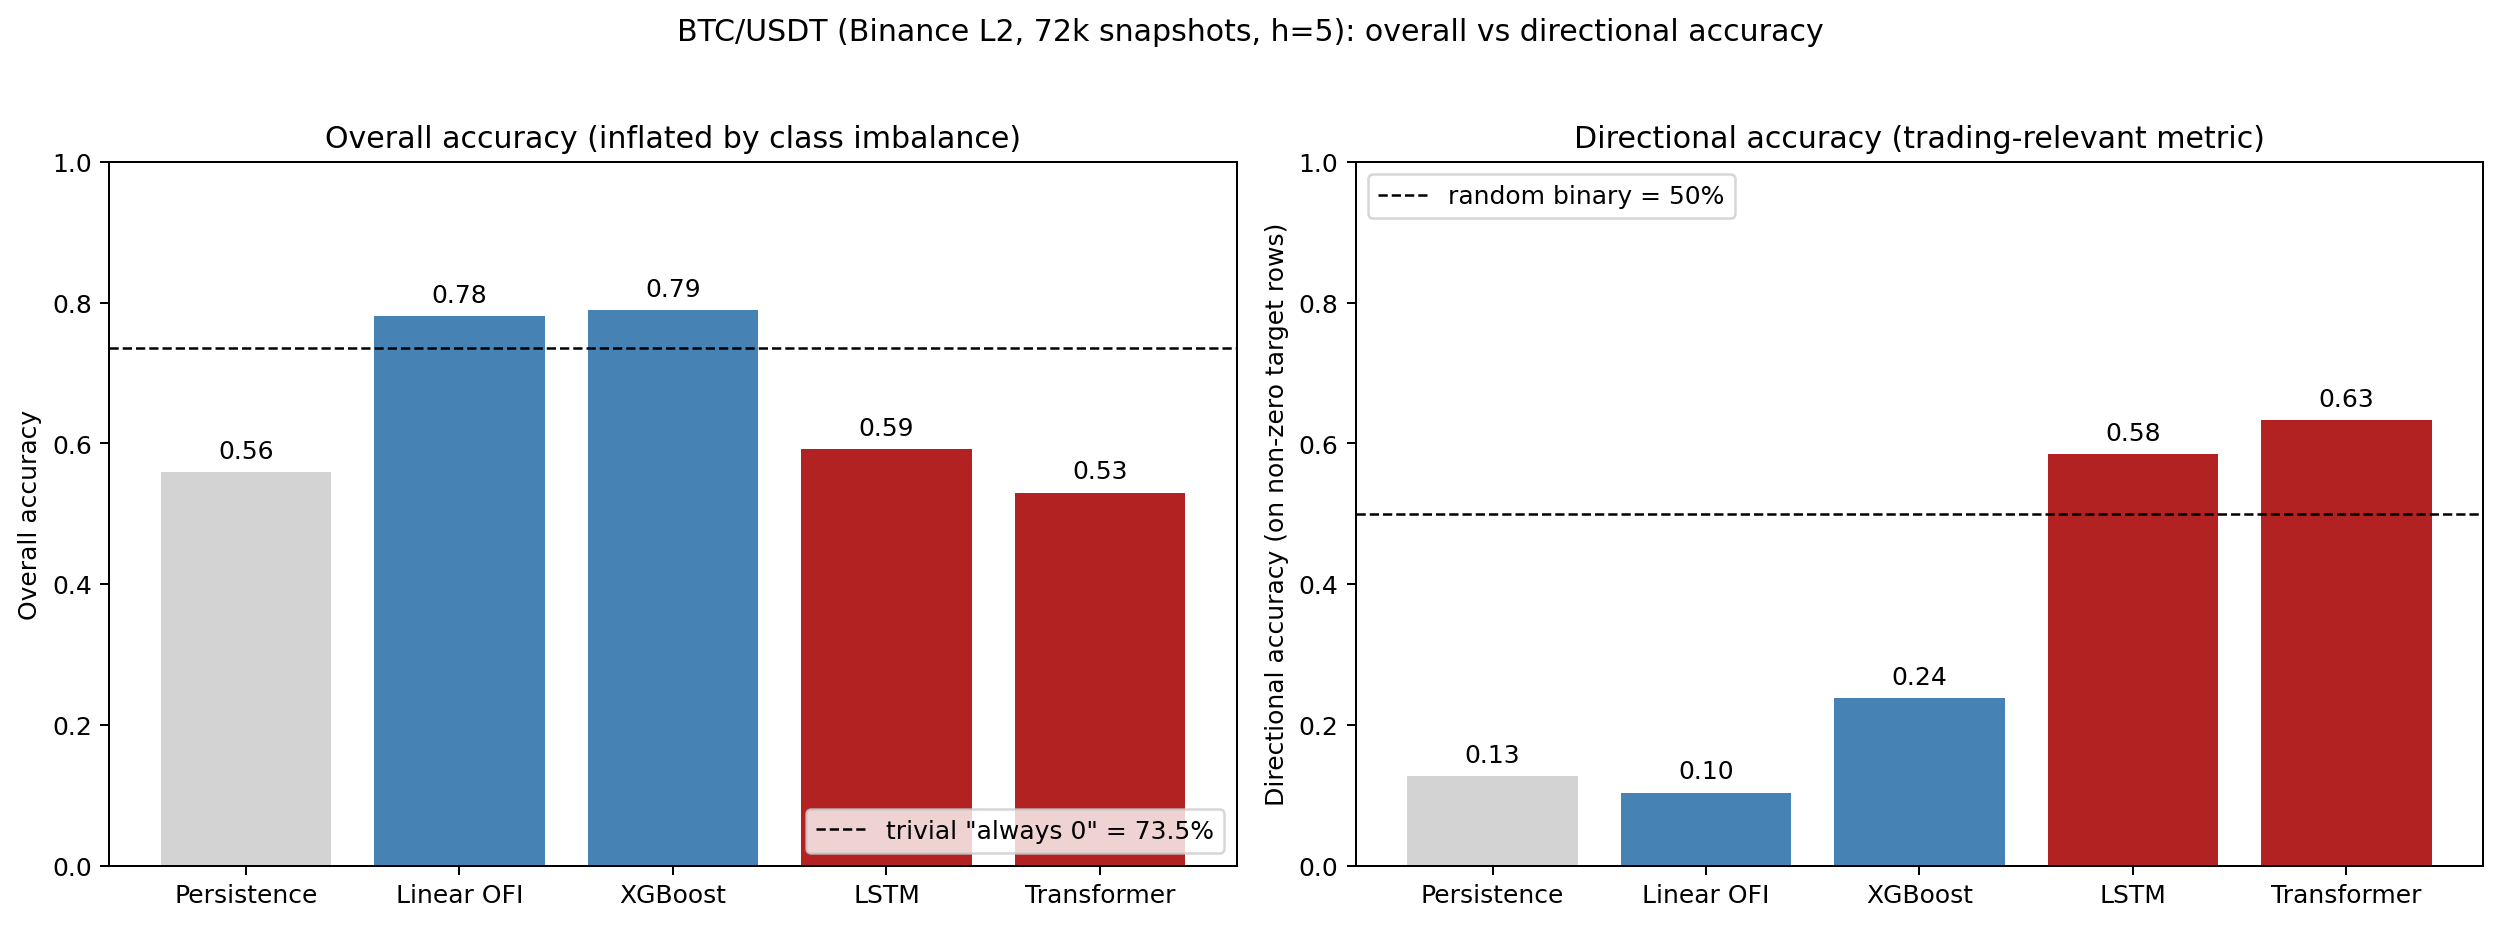
\includegraphics[width=\textwidth]{../results/binance_2h/figures/accuracy_comparison.png}
\caption{Overall accuracy (left, inflated by class-imbalance baseline)
vs directional accuracy (right, the trading-relevant metric). The
two metrics rank models nearly inversely.}
\label{fig:comparison}
\end{figure}

\subsection{Three observations}

\paragraph{Tabular models lean on the dominant class.}
Both linear OFI and XGBoost achieve overall accuracy above 78\%, but
this is only 4.5--5.5 percentage points above the trivial
``always predict 0'' baseline of 73.5\%. Their directional accuracy
on non-zero target rows is correspondingly low: 10.4\% for the
linear model, 23.9\% for XGBoost. The linear model in particular
is \emph{below} the 33\% three-class random baseline, indicating that
when the market actually moves, the linear model is more likely to
predict no-move than the correct direction.

\paragraph{Sequence models trade overall accuracy for directional skill.}
The LSTM and Transformer, trained with class-weighted cross-entropy,
predict non-zero classes more uniformly. Their overall accuracy drops
below the ``always 0'' baseline (LSTM 59.2\%, Transformer 53.0\%), but
their directional accuracy rises substantially: 58.5\% for the LSTM
and 63.3\% for the Transformer, both clearly above the 50\% random
binary baseline.

\paragraph{Transformer dominates LSTM on directional accuracy.}
The Transformer achieves the highest directional accuracy (63.3\%
vs LSTM's 58.5\%, a 4.8 percentage-point gap) despite having lower
overall accuracy. We interpret this as evidence that attention over
the 50-event input window captures specific OFI patterns that
precede directional moves more reliably than the LSTM's
last-hidden-state summary.

\subsection{Persistence is a meaningful floor}

Persistence (predicting the most recent observed direction) achieves
55.9\% overall accuracy---below the ``always 0'' baseline---and only
14.6\% directional accuracy. This confirms it is a useful sanity
floor: any model worth deploying should beat it on at least one
metric, and ideally both.

\section{Discussion}
\label{sec:discussion}

\paragraph{Why does overall accuracy mislead under LOB imbalance?}
For a three-class target where the modal class has base rate
\(p_0 \approx 0.74\), a degenerate ``always predict \(0\)'' classifier
trivially achieves \(p_0\) overall accuracy. A model that puts
non-trivial probability mass on \(\pm 1\) classes will misclassify
some no-move events, paying an accuracy penalty proportional to the
fraction of those events it sends to non-zero predictions. The model
gains accuracy back only by correctly catching the (sparse)
non-zero events. Under heavy imbalance the gains rarely offset the
losses on the overall metric, even though the model has learned
something genuinely useful.

\paragraph{Why does directional accuracy work?}
By restricting evaluation to rows where the target is non-zero,
directional accuracy measures only the metric a trading application
would care about: \emph{given that the market is about to move,
which way?} A model that cannot answer this question above the 50\%
random binary baseline has no trading value regardless of its
headline accuracy. A model that answers it at 60--65\% has
non-trivial directional skill---the precise magnitude that signal
research in this area aims to capture and monetize.

\paragraph{Why do sequence models win directional accuracy?}
The OFI feature panel is local: each row's features are computed
from a single book update or a small rolling window. Tabular models
have access to the same features but treat each prediction
independently. Sequence models, in contrast, can learn temporal
patterns spanning the full 50-event input window---bursts of
imbalance, cancellation cascades, microprice deviations---that
\emph{precede} directional moves. The attention mechanism in the
Transformer appears particularly well-suited to identifying these
temporally distant cues.

\paragraph{Limitations.}
This is a single-asset, single-window study. Generalisation across
symbols, exchanges, and longer time periods is not established here.
The synthetic message file caveat (Section~\ref{sec:data}) means
trade-flow features are not exercised; a future experiment subscribing
to the \texttt{@trade} stream alongside \texttt{@depth} would close
that gap. Hyperparameters are not extensively tuned; sensitivity
analyses on sequence length, hidden size, and refit cadence are
the natural next ablations. Finally, we do not provide statistical
significance tests for pairwise differences in directional accuracy;
this would require a longer capture or multi-asset replication to
have adequate power.

\section{Conclusion}
\label{sec:conclusion}

We benchmarked five model families on a real Binance BTC/USDT level-2
capture. Overall classification accuracy and directional accuracy
on non-zero target rows rank the models nearly inversely: tabular
models (linear, XGBoost) win on overall accuracy by leaning on the
73.5\% no-move dominant class, but achieve only 10--24\% directional
accuracy; sequence models (LSTM, Transformer) trade overall accuracy
for directional skill, achieving 58--63\% directional accuracy. The
Transformer is the clear directional-accuracy leader on this sample.

The methodological takeaway is that practitioners and researchers
evaluating LOB classification models should report both metrics
explicitly: headline accuracy alone systematically prefers
degenerate dominant-class predictors over models with genuine
trading-relevant signal.

\paragraph{Future work.} Natural extensions are: (i) multi-asset
capture across BTC, ETH, SOL to test generalisation; (ii) longer
single-asset captures for statistical power on pairwise comparisons;
(iii) subscribing to the trade stream for genuine event-level
features; (iv) hyperparameter sensitivity analyses for the sequence
models; (v) attention-pattern interpretability to identify which
specific OFI events the Transformer weights highest before
directional moves.

\paragraph{Code and data.} All code, configurations, the captured
Binance dataset, and analysis outputs are available at
\url{https://github.com/manavmishra-cloud/lob-imbalance-signals}.

\bibliographystyle{plainnat}
\bibliography{references}

\end{document}
